\section{High Level Design}
This section of the paper details the top level design of a self encrypting USB based password manager. Various user requirements were identified in the plan of development section of this paper. These included that the design should be: USB based, provide user feedback and should be easy to use. Therefore the design approach adopted is focused at meeting these user requirements and ensuring a modular and isolated design.

\subsection{Design Overview}
Figure 4.1 depicts the block level diagram of the overall system and is seen to consist of a number of hardware and software components. Figure 4.2 is the resulting breadboard implementation. The core of the system consists of two 8-bit microcontroller to handle various data processing tasks as well as USB driver functionality. Three software modules to handle file storage, cryptographic operations as well as high level communications are required and are implemented in firmware. The functionality of each module should be isolated (isolation is a key software security principle). The software client is seen to consist of a browser extension (which provides a GUI to interface with the device) as well as a middle man client (the native host) which communicates with the USB driver microcontroller through a USB based virtual serial (COM) port. A video demonstration of the overall system is shown in \hyperref[sec:SystemOverview]{Appendix A}.

\begin{figure}[H]
\centering
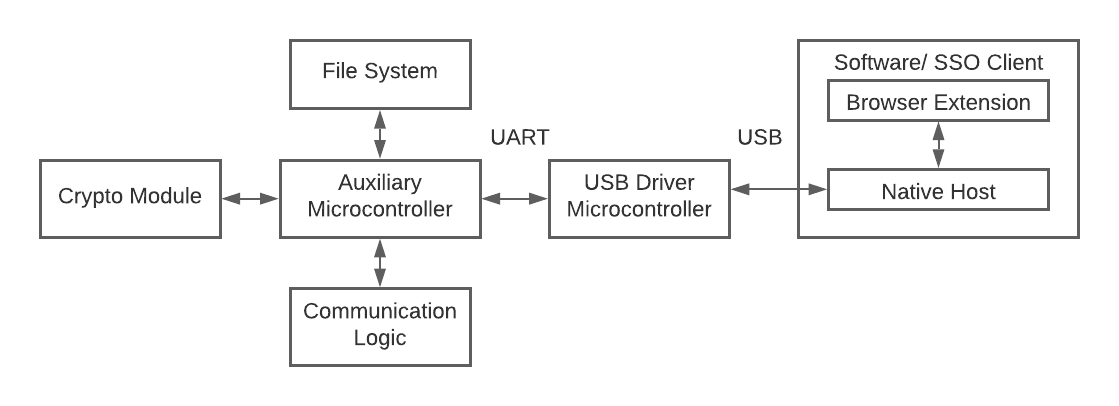
\includegraphics[width=0.9\columnwidth]{Figures/Fig_73.png}
\caption{Block diagram of end system.}
\label{fig:gantt}
\end{figure}

Various design approaches were available when implementing the overall system. For example the cryptographic module could have been offloaded to the software client instead of the microcontroller. This would have most likely resulted in a performance improvement for encryption/decryption operations due to the fact that the clock speed on a modern computer is significantly higher than a crystal driven microcontroller. Another approach could have involved offloading the filesystem to the software client, this would have resulted in significantly more storage space since the EEPROM of most microcontrollers is typically in the KB range. 

\begin{figure}[H]
\centering
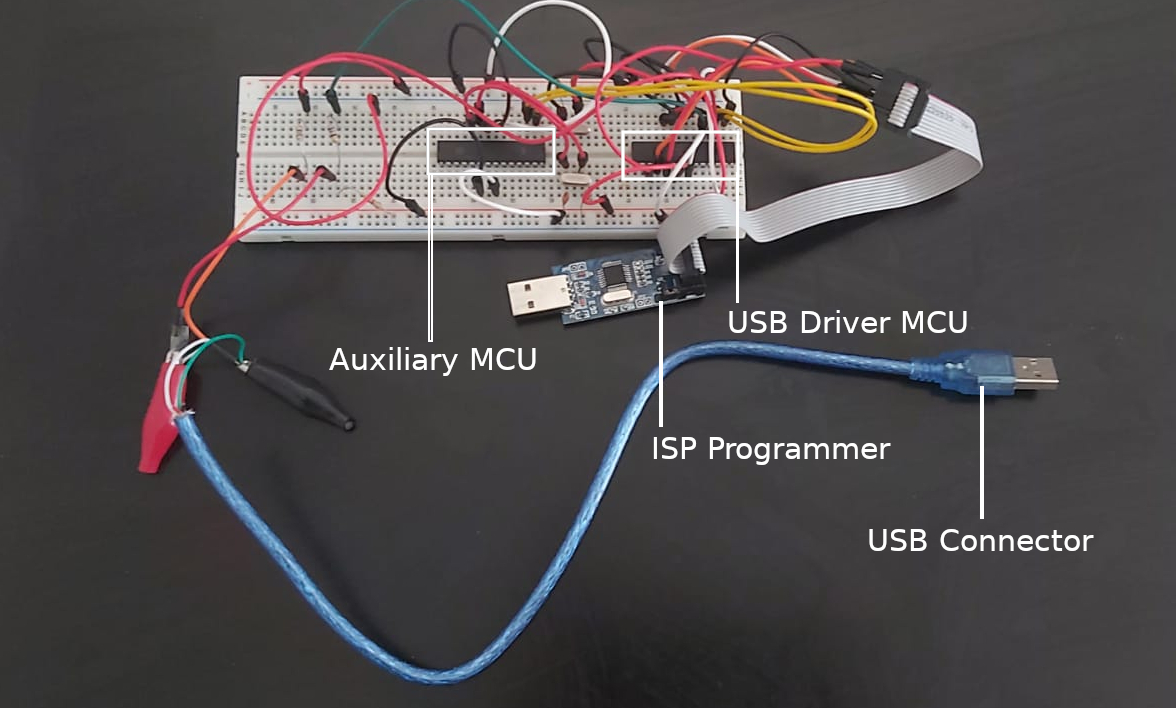
\includegraphics[width=0.9\columnwidth]{Figures/Fig_76.jpeg}
\caption{System prototype overview.}
\label{fig:gantt}
\end{figure}

The approach taken in the design of the firmware based cryptographic module was also important. For example, a choice had to be made whether to implement both encryption and decryption on the microcontroller or offload decryption, for example, to the software client. Since the clock speed of the micro-controller was in the MHz range cryptographic operations would most likely need some time (seconds) to complete. However the aim of this paper was to design a microcontroller based self-encrypting system so some cryptographic functionality should be implemented in hardware where security and performance do not suffer significantly as a result. The resulting design choices and reasoning are addressed in each high level subsystem section. 

The implementation of the software client was another consideration. For example a purely browser based implementation could be considered at the expense of not being able to use various libraries that would otherwise be available in programming languages such as C/C++. This approach would result in a simpler installation procedure, however if various system functionality where to by offloaded to the software client this would imply the use of JavaScript to replicate the same functionality, which for cryptography would involve some sort of performance penalty.

Additionally a USB driver is required to be implemented to facilitate data transmission between the software client and the auxiliary microcontroller over USB. The software client consists of the necessary code to permit a user to securely log onto one or more online accounts and includes a browser client with pseudo SSO capabilities. From the high level description, a table of hardware and software requirements/subsystems was created and is shown in Table 1. It consists of 4 hardware requirements (H01-H04) and 7 software requirements (S01-S07). Each hardware and software subsystem is described in more detail in sections 4.2 and 4.3, resulting design decisions are described in section 4.4.


\begin{table}[H]
\centering

\begin{tabular}{|r|l|}
\hline
\multicolumn{1}{|l|}{\textbf{Requirement}} & \textbf{Description} \\ \hline
H01 & Microcontrollers for data processing and USB driver. \\ \hline
H02 & Hardware to upload programs to microcontroller.\\ \hline
H03-H04 & Circuitry to support the operation of microcontroller. \\ \hline
S01 & Software development environment for firmware and software client.\\ \hline
S02 & Programming languages for firmware and software client development. \\ \hline
S03 & Firmware to support communications between host-client over USB. \\ \hline
S05 & File system implementation in firmware to store credentials. \\ \hline
S06 & Cryptographic implementation in firmware to support encryption. \\  \hline
S07 & Software client to manage credential retrieval and account sign-on.\\ \hline
\end{tabular}
\caption{Software and hardware requirement matrix.}
\label{tbl:HWSWRequirements}
\end{table}
\subsection{Hardware Requirements}
\subsubsection{H01 - Microcontroller }
A microcontroller or MCU (Figure 4.3) generally forms the brains of an embedded system. It generally consists of a processing core and peripherals such memory and static ram. The resulting high level depiction of the overall system shown in Figure 4.1 is seen to consist of a microcontroller-software client interface. The software client will generally be running on another information system such as a computer. Therefore some form of data co-ordination is required, especially since the communications is over USB. Additionally the microcontroller supports file system and cryptographic functionality. 

\begin{figure}[H]
\centering
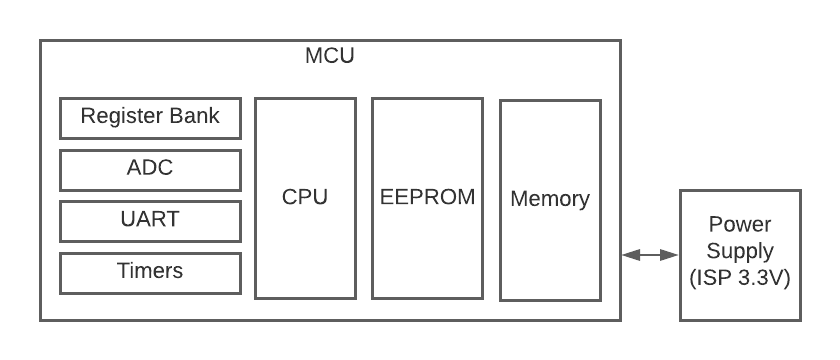
\includegraphics[width=0.8\columnwidth]{Figures/Fig_67.png}
\caption{MCU architecture.}
\label{fig:gantt}
\end{figure}

Two families of microcontroller are commonly used: AVR and PIC. AVR based microcontrollers tend to be cheaper (cost was identified as a core user requirement) and have a wider range of open source hardware programmers to choose from. AVR microcontrollers are also generally more available through local distributors than their PIC counterparts.

Another approach is to use a hardware platform such as a Raspberry PI or Arduino. Some advantages of this approach involve quick prototyping and software development, while some disadvantages include inflexibility when hardware changes are required and the costs involved after component failure. It is still however possible to use some of the technologies bundled with platforms such as Arduino. For example the core bootloader, the software component which enables high level software functionality, can be burned onto an AVR microcontroller. Thus providing the benefits of the Arduino software core while retaining a custom hardware layout. This will be the approach adopted for this project (for the auxiliary microcontroller).


The ATmega and ATtiny are the two primary AVR microcontroller families. Most microcontroller families vary by RAM and EEPROM capacity as well as clock speed. Some common AVR micrcontrollers include the ATtiny45, ATmega8 and ATmega328. The ATmega328P is a good, low cost general purpose microcontroller in widespread circulation. It has 1024B of EEPROM storage, 2KB of SRAM and a typical clock speed of 16MHz. It is also the main microcontroller used in the Arduino Uno which, if acquired, makes software and hardware debugging easier. The hardware characteristics of the ATmega328P make it well suited for software development using programming languages such as C/C++ where memory constraints and overhead are important. The 1024B EEPROM also allows the storage of an acceptable number of user credentials. The use of microcontrollers with less memory or storage capacity might result in performance or technical issues during development.

Two microcontrollers will be utilized for this project. The first is termed the auxiliary microcontroller and is responsible for high level operations such as serial (UART) messaging and encryption, the second microcontroller is responsible for managing USB connectivity and is termed the USB driver MCU.

\subsubsection{H02 - ISP Programmer }
A microcontroller would not be of much use if we could not upload custom firmware. The solution to this problem is in the widely supported ISP (in-system programming) capability of modern microcontrollers. This requires the use of an ISP compatible programmer which are often USB based. The choice of ISP programmers is generally not too critical however due to budget constraints, a cheap solution is ideal. The USBasp is an open source and widely available AVR programmer.  Other AVR ISP programmers include the USBtiny and AVRISP mkII. The Arduino Uno can also be used as an ISP programmer.
\subsubsection{H03 - Crystal Oscillator }
Modern microcontrollers will typically support both an internal and external clock source. Internal clock sources for most low cost microcontrollers however tend to be rather slow with poor stability and typically an external clock is recommended. A crystal oscillator utilizes the mechanical resonance of a piezoelectric material in order achieve oscillation. They typically perform well as oscillators for their price.

The choice of crystal frequency to use depends on a number of factors. One important consideration is the required clock speed of the USB driver implementation. A low speed USB device needs to transfer at a rate of 1.5Mb/s \cite{usb_speed}. Another consideration is the list of supported crystal frequencies used by the USB driver implementation. Since the USB driver uses the V-USB software stack the choice of crystal frequencies will be limited to 12,15,16,18 and 20MHz \cite{vusb}. 16MHz is a common value for the ATmega328. A few MHz difference would not effect performance that much.

\subsubsection{H04 - Passives }
In order to support the freestanding operation of a microcontroller, that is without using a prepackaged solution such as a raspberry PI or an Arduino, various passive components such as resistors and capacitors are required in order to set up a stable clock and feed control lines the correct amount of current. Various types of resistors are available include wire wound and carbon film resistors. The choice of resistors isn't too important for low speed applications but becomes more critical at higher frequencies, such as at RF.
\subsection{Software Requirements}
\subsubsection{S01 - Software Development Environment}
A suitable development environment is required in order to develop the system firmware for the microcontroller as well as the browser based software client. A development environment typically consists of an IDE (integrated development environment) and a series of compilers. Various IDE's are available including: Atom, Visual Studio, Visual Studio Code. A development environment also typically consists of the necessary hardware to support the end user in developing the required software. The hardware platform used during development of the end system (writing code, flashing) as well as writing of the report is shown in Table 2. 

\begin{table}[]
\centering

\begin{tabular}{|r|l|}
\hline
\multicolumn{1}{|l|}{\textbf{Specification}} & \textbf{Description} \\ \hline
OS & Ubuntu 20.04.1 LTS Linux 64-bit. \\ \hline
CPU & 3.5GHz Dual-Core AMD Athlon 3000G.\\ \hline
RAM & 8GB-DDR3. \\ \hline
SSD & 500GB SATA.\\ \hline
Motherboard & Gigabyte A320M-S2H-CF. \\ \hline
\end{tabular}
\caption{Hardware specifications of personal computer.}
\label{tbl:HWSWRequirements}
\end{table}

\subsubsection{S02 - Programming Language}
Various programming languages exist and are suitable for use in developing system firmware as well as software for the web. Often low level programming languages are compiled into native object code while higher level languages are typically interpreted. Developing firmware typically requires the use of a low level language while developing computer software is most time efficient when utilizing higher level languages. C/C++ are popular choices for firmware and system level programming while JavaScript is more suited to developing browser based software. Webassembly is another alternative to JavaScript and is a recent specification that allows developers to compile their C/C++ programs into WebAssembly binaries that can be executed from a browser. Most browsers now support the WebAssembly specification.

\subsubsection{S03 - USB Driver}

In order to facilitate communication between the auxiliary MCU and client software a USB driver implementation must be developed for the microcontroller. USB is a complex protocol and various open source driver implementations exist for various microcontroller manufacturers.

Figure 4.4 depicts the flow of data from a microcontroller to the software client and vice versa. The auxiliary microcontroller is responsible for formatting serial messages to be sent over USB in response to commands issued by the software client. An example of a message sent from the auxiliary MCU to software client might be the contents of a file (encrypted credential) requested by the software client for decryption. The formatted messages are passed on to the the USB driver MCU (through UART) which then transfers the message over the USB bus where it is intercepted by the software client through a virtual serial (COM) port.

\begin{figure}[]
\centering
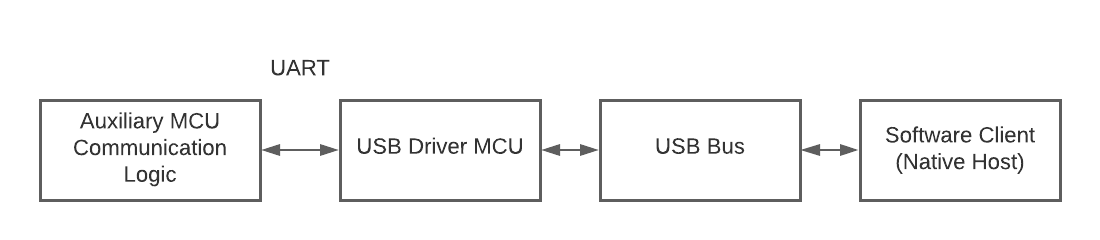
\includegraphics[width=0.85\columnwidth]{Figures/Fig_74.png}
\caption{USB communication pathway from host to software client.}
\label{fig:gantt}
\end{figure}

Various options exist for USB based communications. One popular approach is to use a USB to serial converter board such as the CP2102. These boards typically integrate logic to convert between USB based communication and the UART specification. One advantage to this approach is that enabling USB based communication for a particular embedded system becomes easy and straightforward. Another advantage is that for kernels such as Linux no drivers are required to be installed in order to communicate with an MCU. One disadvantage however is that the converter boards are typically more expensive than implementing USB functionality oneself (using a microcontroller).

Another approach is to use an open source USB driver and implement USB driver functionality within a microcontroller itself. Various open source USB driver implementations exist. For AVR based microcontrollers the V-USB \cite{vusb} driver provides low speed (1.5Mb/s) USB emulation. Three main USB classes exist, namely CDC, HID and MSC. In CDC, communication device class, mode a USB connection behaves very similar to a typical RS232 serial channel. A virtual COM (communications) port is opened on the host operating system. For linux connections are typically seen as /dev/ttyACM* for the ACM (abstract control model) mode of CDC. 

A HID, human interface device, class USB device typically represents hardware such as mice, keyboards and display devices and is used to transfer data from a host device to an endpoint such as an operating system. Data usually flows in one direction in this mode, outward from the host device to an endpoint. It can however be used as a bidirectional communications channel but this is not ideal. Finally MSC, mass storage class, is similar in operation to CDC mode but sees a file system instead of utilizing simple commands to send data.

USB CDC emulation using an open source driver such as USB-V is ideal because sending and receiving data is relatively straightforward, only requiring reading and writing to /dev/ttyACM* in Linux and no specific drivers are needed in order to recognise a USB CDC host. One disadvantage to this approach is that a dedicated microcontroller is needed for USB communication and due to the timing requirements of USB the same microcontroller cannot be used for much else, thus requiring two microcontrollers for a typical embedded application.

The approach taken in the design of the USB driver interface will be to implement a CDC ACM class device on the USB driver MCU. This is due to the fact that CDC ACM is a widely supported standard among both the Windows and Linux kernels and allows the emulation of a serial channel through which a variety of Arduino compatible libraries can be used for serial communication on the auxiliary MCU. 

\subsubsection{S04 - File System}
A file system implementation is required in order to store and retrieve data such as encrypted user credentials. Various file system specifications exist, such as FAT, NTFS and EXT3. However for the purposes of this paper a custom file system will be developed. The reasons for this are that existing file systems provide complex functionality that is not required for our end system. Rather a flat file system with basic functionality which supports file encryption/decryption and uses the EEPROM of microcontrollers is ideal.

An alternative approach may involve not utilizing a file system at all, but storing information in a linear manner within EEPROM and keeping track of data offsets. This has the advantage of being simple to implement but has no structure, so managing file data over time might become complex. Therefore a file system becomes critical as the size of data increases.

Figure 4.5 depicts a high level overview of the required file system functionality. It is seen to consist of an API that supports file read, write and delete operations. File operations directly effect the storage medium (EEPROM) and the file system API supports the enumeration of existing files (List). The API shown in Figure 4.5 is the basis for any filesystem type.

\begin{figure}[H]
\centering
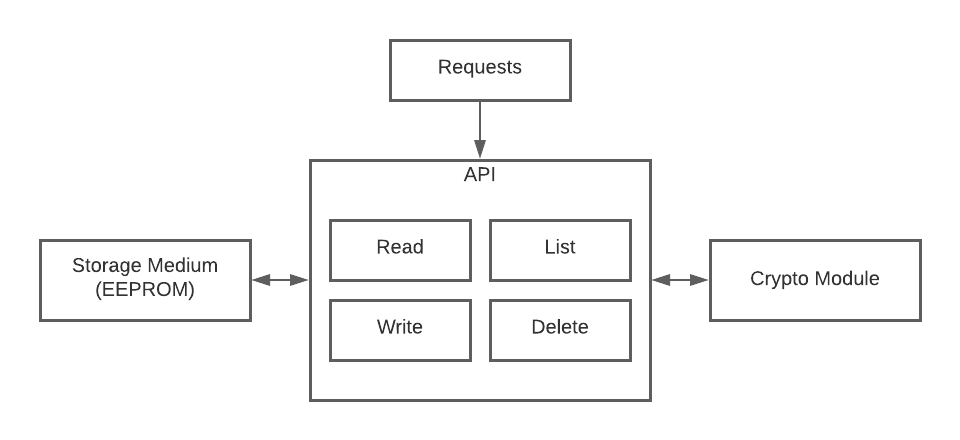
\includegraphics[width=0.8\columnwidth]{Figures/Fig_20.png}
\caption{File system API.}
\label{fig:gantt}
\end{figure}
\subsubsection{S05 - Crypto Module}
The crypto module is responsible for providing the necessary cryptographic functionality to insure the secure transmission and storage of credentials. Various design approaches are possible for the cryptographic functionality of the host device. The first important consideration was the actual encryption algorithm to use. In the literature review AES as well as RSA were investigated. The requirements for the selection of an encryption algorithm mainly centered around ease of implementation. Since the data being encrypted was small in size, memory and typical performance characteristics were not deemed as important.

After researching various code implementations of AES and RSA, it was decided that RSA would be the most straightforward to implement from scratch. RSA only requires that multiplication and modulo arithmetic be implemented on the host for encryption compared to AES which requires state transformations (expansion, shift. mix, etc). In respect to security considerations, RSA is still regarded as providing adequate security given that a sufficiently large key modulus is used. A trade-off of RSA key size to performance must typically be made for embedded systems.

Another factor to consider was whether the host device (MCU) should implement both encryption and decryption functionality or if either process should be offloaded to the software client. One approach may involve implementing decryption on the host device and encryption on the software client. This approach is flawed since RSA decryption is significantly slower than encryption for small public exponents (i.e e=3) \cite{rsa_speed}. A better approach may involve implementing encryption on the host device and decryption on the software client.

Given the hardware limitations of most microcontrollers, and that RSA is an asymmetric algorithm implementing both encryption and decryption on the host device might result in unacceptable performance metrics. So offloading one of these cryptographic processes is ideal, specifically decryption. Figure 4.6 is a high level representation of the crypto API. 
\begin{figure}[H]
\centering
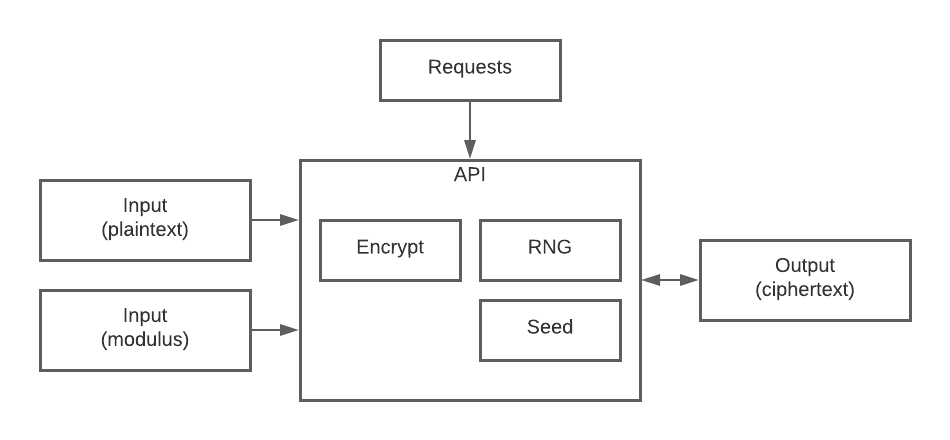
\includegraphics[width=0.8\columnwidth]{Figures/Fig_21.png}
\caption{Cryptographic API.}
\label{fig:gantt}
\end{figure}

It is seen consisting of encryption functionality (Encrypt) as well as a RNG (random number generator) to assist with encryption padding. This RNG may be seeded by a random initial value, such as the voltage of a floating pin in order to insure randomness and different output ciphertext for the same input plain-text.

The encrypt functionality is seen taking two inputs, the corresponding plain-text password as well as key modulus. The choice then of the public key exponent as well as number of bits of the modulus becomes a critical component of the overall encryption scheme. In terms of the public key exponent typical values are 3 or 65537. The choice between the two has an impact on performance, however assuming proper padding the choice of public exponent should theoretically not impact security \cite{exponent}. The number of bits of the modulus(n) also has an impact on security. A modulus of 512 bits, 1024 bits and 2048 bits can be found in many embedded system implementations. However RSA-512 has been deprecated and is susceptible to brute force attacks. RSA-1024 has not yet been factorized \cite{fact2} and offers a performance improvement over RSA-2048 especially for resource constrained embedded systems.

\subsubsection{S06 - Communication Logic}
Communication between the auxiliary microcontroller and software client over serial (at a high level) is delegated by various software logic. This is required to be implemented on either side of the communications chain (Figure 4.7). The auxiliary MCU is responsible for monitoring the serial line for commands, extracting variables (through command unpacking) and returning results to the software client over the serial connection. The software client is responsible for formatting/packing commands to be sent over serial (in the format specified in section 5.4.1) requested by the browser extension component of the software client. The serial connection between these two endpoints should also be transparent to USB (handled by the USB driver MCU).
\begin{figure}[H]
\centering
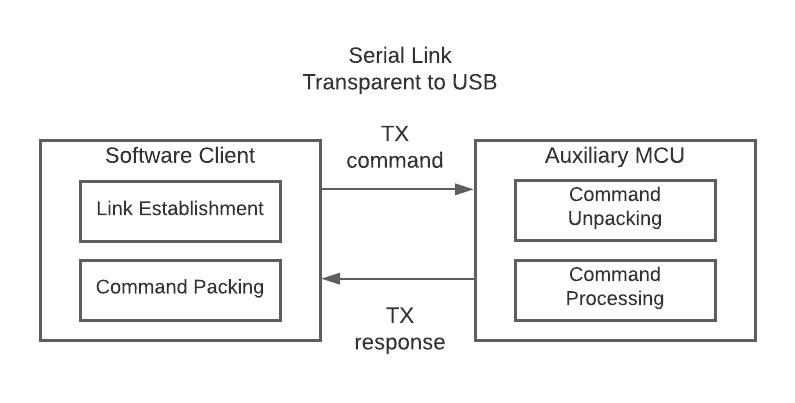
\includegraphics[width=0.7\columnwidth]{Figures/Fig_75.png}
\caption{Communications Logic.}
\label{fig:gantt}
\end{figure}
 
 Commands (sent from the software client to auxiliary microcontroller) should be sent as one long string over the active serial connection. For example given an encryption event the software client would send the modulus and data to be encrypted at once. The choice in this approach is due to the fact that the maximum length of a command is smaller than the maximum memory capacity (RAM) of the ATmega328P (approx 2KB).

\subsubsection{S07 - Software Client}
 Figure 4.8 depicts a high level overview of the software client. It is seen to consist of a browser extension and native host (middleman) client which both run on a host PC. The browser extension is responsible for SSO functionality as well as adding and fetching online credentials. The native host is responsible for decrypting credentials as well as formatting serial commands to be sent the the USB driver MCU. 

Additionally the native host supports the generation of RSA cryptographic keys to be used in the encryption and decryption of credentials. These keys are stored in a database on the software client of the end user. It is important to maintain the secrecy of these keys in order to avoid credential compromise. These credentials are isolated from the MCU in order to avoid key extraction techniques from the EEPROM based file system.
\begin{figure}[H]
\centering
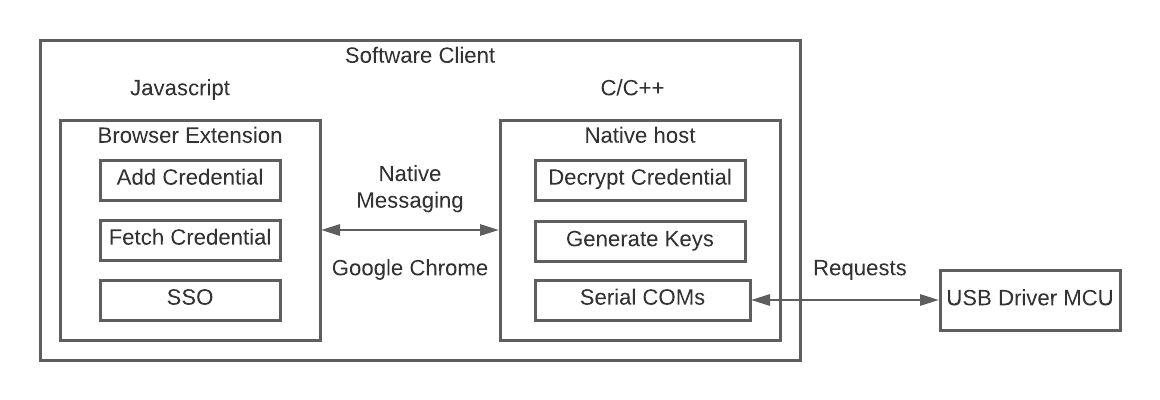
\includegraphics[width=1\columnwidth]{Figures/Fig_59.png}
\caption{Software client overview.}
\label{fig:gantt}
\end{figure}

Since key generation as well as decryption is handled by the software client, the performance of the overall system should only be limited by the encryption time of credentials on the auxiliary MCU. Another important consideration was the method of communication with the host browser and software client in order to enable SSO capability. For example google chrome supports inter-process communication using it's native messaging API \cite{native_messaging}, another alternative is using WebSockets. Here a WebSocket server is spawned on the software client and a connection to the server made through a browser plugin. 

The positioning of the credential database is also important. One approach may involve using a browsers local storage facility. One advantage to this approach is that credential storage becomes seamless to a web browser extension. However implementing credential storage from the browser may expose the database to all the inherent security vulnerabilities that come with web storage.  Alternatively the credentials could be stored as a file (in the users home directory for example). This has the advantage of isolating sensitive information from the browser but at the cost of requiring the exchange of credential information with the software client which is vulnerable to various attack vectors as outlined in the literature review. 

Since decryption and key generation is handled by the software client, the relevant libraries to use becomes important. Since the software client will be written in C/C++ various cryptography libraries are available including: libtomcrypt, Crypto++ as well as OpenSSL. OpenSSL is a widely used cryptography library that supports a wide range of ciphers including: AES, Blowfish, RC4 and RSA. It is a FIPS 140 certified \cite{fips} cryptographic library so it's RNG and RSA implementations have been tested extensively. 

\subsection{Design Decisions}

After careful consideration of the various advantages and disadvantages of the options available for each requirement, a table of design decisions was created (Table 3).

\begin{table}[H]
\centering
\resizebox{0.85\textwidth}{!}{%
\begin{tabular}{|l|l|l|}
\hline
\textbf{Requirement} & \textbf{Description} & \textbf{Decision} \\ \hline
H01 & \begin{tabular}[c]{@{}l@{}}Microcontrollers for data processing\end{tabular} & ATMega328P\\ \hline
H02 & \begin{tabular}[c]{@{}l@{}}Hardware to upload \\  programs to microcontroller\end{tabular} & USBasp ISP \\ \hline
H03 & \begin{tabular}[c]{@{}l@{}}Cystal Oscillator \end{tabular} & 16 MHz \\ \hline
H04 & \begin{tabular}[c]{@{}l@{}}Passives\end{tabular} & Resistors, Capacitors \\ \hline
S01 & Software Development environment & \begin{tabular}[c]{@{}l@{}}Visual Studio Code\\ AVR-GCC\end{tabular} \\ \hline
S02 & Programming Languages & \begin{tabular}[c]{@{}l@{}}C/C++, Javascript\end{tabular} \\ \hline
S03 & \begin{tabular}[c]{@{}l@{}}USB Driver\end{tabular} & V-USB CDC  \\ \hline
S04 & \begin{tabular}[c]{@{}l@{}}File System\end{tabular} & Custom \\ \hline
S05 & \begin{tabular}[c]{@{}l@{}}Encryption Algorithm\end{tabular} & RSA-1024 \\ \hline
S05 & \begin{tabular}[c]{@{}l@{}}Cryptography Library (Decryption, Keygen)\end{tabular} & OpenSSL \\ \hline

\end{tabular}
}
\caption{Design Decisions}
\label{tbl:DesignDecisions}
\end{table}

